\pagebreak

\section{Caminata aleatoria}

El concepto de random walk comenzó en 1827 cuando el botánico Robert Brown
estudió el movimiento del polen. También es importante la aportación de Albert
Einstein de 1905 sobre el movimiento browniano de pequeñas partículas.

Una caminata aleatoria simple sobre el conjunto de números enteros $\mathbb{Z}$
es un proceso estocástico a tiempo discreto $X_n : n=0,1, ...$ que evoluciona de
la siguiente forma: iniciando en el estado 0, al tiempo 1 el proceso puede pasar
al estado 1 con probabilidad $p$, o al estado 1 con probabilidad $q$, en donde
$p+q=1$. Se usa la misma regla para los siguientes tiempos, es decir, estando en
el estado $k$, al siguiente instante el proceso pasa al estado $k+1$ con
probabilidad $p$, o al estado $k-1$ con probabilidad $q$. El valor de $X_n$ es
el estado donde se encuentra el proceso al tiempo n y puede escribirse como

\begin{equation}
    X_n = \xi_1 + \xi_2 + ... + \xi_n,
\end{equation}

en donde $\xi_1, \xi_2,...$  es una sucesión de variables aleatorias
independientes con idéntica distribución

\begin{equation}
    P(\xi=+1) = p
\end{equation}
\begin{equation}
    P(\xi=-1) = q = 1-p
\end{equation}

\begin{figure}[h!]
    \centering
    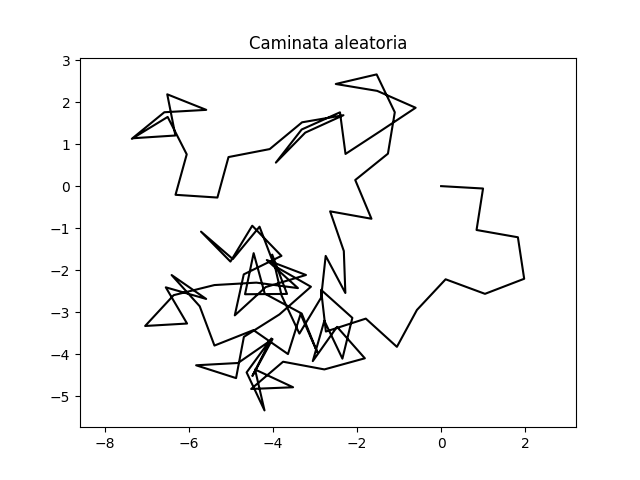
\includegraphics[scale=0.8]{figures/Random_walk.png}
    \caption{Caminata aleatoria en dos dimensiones.}
\end{figure}

La independencia de las variables aleatorias $\xi_1, \xi_2,...$ tiene como
consecuencia que la caminata aleatoria simple cumpla la propiedad de Markov y
que sea un proceso estocástico con incrementos independientes y estacionarios.
En términos generales el objetivo es estudiar el comportamiento de la v.a. $X_n$
al paso del tiempo. Uno de los elementos fundamentales para estudiar a las
caminatas aleatorias está dado por las probabilidades de transición. Para
cualesquiera enteros $i$ y $j$, las probabilidades de transición en un paso de
la caminata aleatoria simple son:

\begin{equation}
    P(X_{n+1}=j | X_n = i) = \left\lbrace \begin{array}{ll}
        p & \text{si} j = i+1 \\
        q & \text{si} j = i-1 \\
        0 & \text{en otro caso}
    \end{array}\right.
\end{equation}

Como estas probabilidades no dependen de n, se dice que son homogéneas en el
tiempo, es decir, son las mismas para cualquier valor de n. Pueden consi-
derarse también caminatas aleatorias que inician en cualquier valor entero o que
permiten saltar de un estado en sí mismo al siguiente instante (es decir, no
cambiar de estado), o bien, que los saltos no sean unitarios ni los tiempos en
los que efectúan los saltos sean necesariamente tiempos enteros, e incluso
pueden definirse caminatas en dimensiones mayores, por ejemplo, en Z 2 . Las
caminatas aleatorias son procesos que pueden representar versiones discretas de
procesos a tiempo continuo más complejos.

\section{Cadenas de Markov}

Este tipo de procesos es también de amplia aplicación y se cuenta con una teoría
matemática bastante desarrollada.

\begin{theorem}{Cadena de Markov}
Una cadena de Markov es un proceso estocástico a tiempo discreto ${X_n : n=0,
1,...}$ con espacio de estados discreto y tal que 0 y satisface la propiedad de
Markov, esto es, para cualquier entero $n \geq 0$ cualesquiera estados $x_0 , x_1 , . . .
, x_{n+1}$ se cumple la identidad:

\begin{equation}
    \begin{array}{l}
    P(X_{n+1} =  x_{n+1} | X_n = x_n, ..., X_1 = x_1, X_0=x_0) \\
    P(X_{n+1} = x_{n+1} = x_{n+1} | X_n = x_n).
    \end{array}
\end{equation}

\end{theorem}


A las probabilidades condicionales mencionadas en la definición anterior se les
llama probabilidades de transición del tiempo $n$ al tiempo $n+1$, y se les
denota por $p_{x_n, x_{n+1}}(n, n +1)$. Adicionalmente, se dice que la cadena es
estacionaria u homogénea en el tiempo si estas probabilidades no dependen
explícitamente de los tiempos particulares $n$ y $n+1$, sino únicamente de los
estados involucrados. De esta forma, si de manera general se considera la
probabilidad de transición del estado $i$ al estado $j$ de una unidad de tiempo
cualquiera a la siguiente unidad de tiempo, la probabilidad de transición del
primer estado al segundo se escribe como $p_{ij}$ , o $p_{ij}(1)$ , o también
como $p_{ij}^{1}$, es decir, sin importar el valor del entero $n$:

\begin{equation}
    p_{ij} = P(X_n = j | X_{n-1} = i)
\end{equation}

A estas probabilidades se les llama probabilidades de transición en un paso. En
general se considera como espacio de estados para una cadena de Markov el
conjunto discreto $0, 1, ...$ o algún subconjunto finito de él. Haciendo variar
los valores de los índices $i$ y $j$ en este espacio de estados se forma la
matriz de probabilidades de transición en un paso:

\begin{equation}
    P = \begin{pmatrix}
        p_{00}  & p_{01}    & p_{02}    & ... \\
        p_{10}  & p_{11}    & p_{12}    & ... \\
        p_{10}  & p_{21}    & p_{22}    & ... \\
        .       & .         & .         &     \\
        .       & .         & .         &     \\
        .       & .         & .         &
    \end{pmatrix}
\end{equation}
